\chapter{Výsledky pozorovaní}
\label{vysledky}

Predmetom nášho skúmania je vplyv implementácie syntetického gradientu na proces trénovania MMD-ResNet. Predovšetkým sme sa zamerali na pozorovanie vývoja hodnoty MMD počas trénovania MMD-ResNet. Pozorované správanie, resp. priebeh trénovania MMD-ResNet využívajúcej metódu syntetického gradientu sme porovnávali so správaním MMD-ResNet využívajúcej metódu spätného šírenia chyby.

Pri implementácii MMD-ResNet s využitím metódy syntetického gradientu sme sa snažili dodržať pôvodnú konfiguráciu MMD-ResNet (počet reziduálnych blokov, počet kumulovaných vrstiev, hodnota kroku učenia a pod.). Dodržaním pôvodnej konfigurácie je umožnené vykonávať presnejšie porovnania pôvodného modelu MMD-ResNet s modelom MMD-ResNet využívajúcim metódu syntetického gradientu.

Pozorovaná reziduálna sieť MMD-ResNet pozostáva z jednej vstupnej vrstvy, jednej výstupnej vrstvy a troch reziduálnych blokov. Každý reziduálny blok obsahuje dve kumulované vrstvy vykonávajúce dávkovú normalizáciu, transformáciu vstupných dát aktivačnou funkciou ReLU \cite{Goh1995} a váhovanie (viac v Kap. \ref{navrh} a v Kap. \ref{implementacia}). Každá kumulovaná vrstva MMD-ResNet využíva na úpravu váh výhradne syntetický gradient generovaný prislúchajúcim modulom syntetického gradientu. Moduly syntetického gradientu pozostávajú z jednej skrytej vrstvy.

Kumulované vrstvy reziduálnych blokov implementujú $l_2$ regularizáciu hodnôt váh s hodnotou $l_2$ regularizácie $10^{-2}$. Pri trénovaní MMD-ResNet je použitá trénovacia dávka s veľkosťou 1000 buniek. Krok učenia je upravovaný dynamicky, použitím rozvrhu definovaného ako 
\[
    \alpha_t = \alpha_0 . \gamma^{\lfloor\frac{1+t}{T}\rfloor}
\]
kde $\alpha_0$ je počiatočná hodnota kroku učenia, $\gamma$ je predom definovaná konštanta, $t$ je aktuálna iterácia trénovania a $T$ je zvolený rozvrh. V našom prípade sme ako počiatočnú hodnotu kroku učenia $\alpha_0$ použili $10^{-4}$, konštanta $\gamma$ má hodnotu $0.1$ a hodnota rozvrhu $T$ je 50.

\section{Prvé výsledky}
\label{prve_vysledky}

Po implementácii MMD-ResNet využívajúcej metódu syntetického gradientu sme potrebovali zistiť, či je implementácia korektná a či MMD-ResNet svojím trénovaním znižuje hodnotu MMD medzi zdrojovou vzorkou a referenčnou vzorkou. Testovanie sme vykonali tak, že sme inicializovali hodnotu kroku učenia na vysoké číslo ($10^{-2}$) a deaktivovali dynamickú zmenu kroku učenia. Po dokončení trénovania bola reziduálna sieť síce pretrénovaná ale podarilo sa nám dokázať, že hodnota MMD medzi referenčnou a zdrojovou vzorkou má v jednotlivých iteráciách trénovania klesajúci trend (viď. Obr \ref{vysledok1}). Znižovanie hodnoty MMD medzi referenčnou vzorkou a zdrojovou vzorkou predstavuje znižovanie rozdielu medzi distribúciami hodnôt markerov v daných vzorkách.

\begin{figure}
%vlozenie samotneho obrazku vycentrovaneho a vhodnej velkosti
%obrazok je v subore images/cervik.png
\centerline{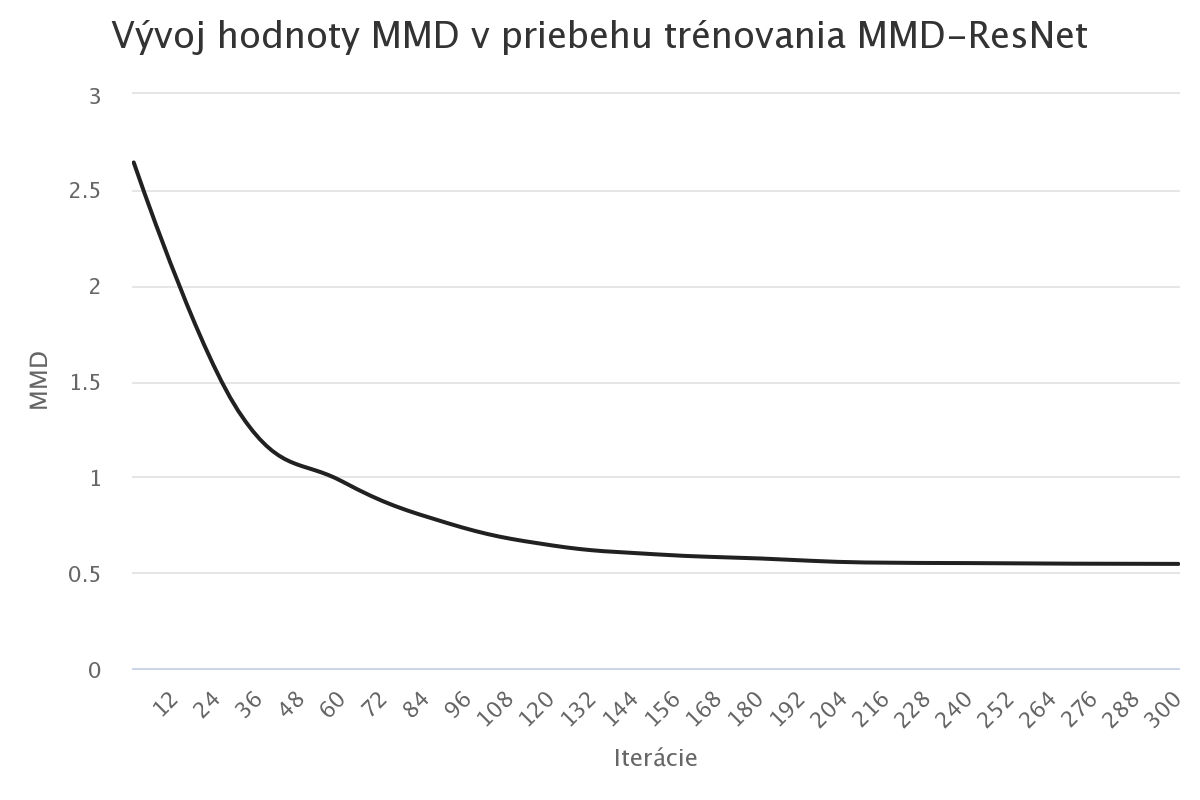
\includegraphics[width=0.7\textwidth]{images/experimenty/experiment1.png}}
%popis obrazku
\caption[Vývoj hodnoty MMD v priebehu trénovania MMD-ResNet]{Graf na obrázku opisuje vývoj hodnoty MMD medzi zdrojovou vzorkou a referenčnou vzorkou v jednotlivých iteráciách trénovania MMD-ResNet. Pri trénovaní bola použitá vysoká hodnota kroku učenia ($10^{-2}$) a dynamická zmena kroku učenia bola deaktivovaná.}
%id obrazku, pomocou ktoreho sa budeme na obrazok odvolavat
\label{vysledok1}
\end{figure}

Experiment preukázal, že reziduálna sieť využívajúca metódu syntetického gradientu ako alternatívu za metódu spätného šírenia chyby je svojím trénovaním schopná znižovať hodnotu chybovej funkcie za predpokladu správnej implementácie.

Zdroj \cite{Jaderberg2016} uviedol, že implementácia syntetického gradientu v neurónových sieťach umožňuje paralelné trénovanie jednotlivých skrytých vrstiev danej neurónovej siete. Výsledkom čoho je zníženie času potrebného na trénovanie neurónovej siete. V našom ďalšom experimente sme pozorovali vplyv implementácie syntetického gradientu v MMD-ResNet na rýchlosť trénovania danej neurónovej siete. 

V Kap. \ref{implementacia_trenovania_MMD_ResNet} sme uviedli, že naša implementácia modelu MMD-ResNet zabezpečuje paralelné vykonávanie optimalizátorov podieľajúcich sa na trénovaní jednotlivých vrstiev MMD-ResNet. Optimalizátory predstavujú matematické transformácie a operácie, ktoré sú zadeklarované pri spustení skriptu a následne vykonávané volaním funkcie \mintinline{Python}{run()}, obsiahnutej v knižnici \mintinline{Python}{TensorFlow}. Výsledky pozorovania dĺžky trvania trénovania MMD-ResNet metódou syntetického gradientu sme porovnávali s dĺžkou trvania trénovania MMD-ResNet metódou spätného šírenia chyby. 

Prvotne sme daný experiment vykonávali na osobnom počítači s využitím výkonu centrálnej procesorovej jednotky (CPU, z angl. Central Processing Unit). Výsledky experimentu opisuje tabuľka \ref{vysledok2}. Trénovanie MMD-ResNet s využitím metódy syntetického gradientu na procesore osobného počítača zabralo viacej času ako trénovanie MMD-ResNet metódou spätného šírenia chyby. Daný výsledok je zapríčinený obmedzením procesorového času pre jednotlivé procesy vykonávané na procesore počítača, vynúteného operačným systémom. Preto trénovanie vrstiev MMD-ResNet využívajúcej metódu syntetického gradientu nebolo realizované paralelne ale sériovo. Vzhľadom k tomu, že v tomto prípade boli obidva modely trénované sériovo, tak trénovanie MMD-ResNet metódou syntetického gradientu trvalo dlhšie, pretože daná metóda vyžaduje trénovanie nie len skrytých vrstiev ale aj všetkých modulov syntetického gradientu.

\begin{table}
% v tabulke sa popis zvykne davat nad tabulku
\caption[Trénovanie MMD-ResNet na procesore počítača]{Tabuľka opisuje dĺžku trvania trénovania MMD-ResNet využívajúcej metódu syntetického gradientu a MMD-ResNet využívajúcej metódu spätného šírenia chyby. Pozorovanie je realizované na 500 iteráciách. Obidva modely MMD-ResNet boli trénované na procesore osobného počítača.}
%id tabulky
\label{vysledok2}
% tu zacina samotna tabulka
\begin{center}
\begin{tabular}{|c|c|c|}
\hline
  & \textbf{Metóda} & \textbf{Metóda} \\
  & \textbf{syntetického gradientu} & \textbf{spätného šírenia chyby} \\
\hline
\textbf{Počet iterácií} & 500 & 500 \\
\hline
\textbf{Čas} & 567s & 513s \\
\hline
%(many lines omitted)
\end{tabular}%
\end{center}
\end{table}

Obmedzenia procesorového času operačným systémom sa nevzťahuje na procesorový čas grafických akcelerátorov. Preto sme sa daný problém rozhodli riešiť realizáciou trénovania MMD-ResNet na grafických akcelerátoroch. Trénovanie sme vykonávali v prostredí webovej služby Google Colaboratory. Ako sme uviedli v Kap. \ref{uprava_implementacie_ResNet}, služba Google Colaboratory umožňuje bezplatné trénovanie neurónových sieti na grafických akcelerátoroch. Spustením trénovania MMD-ResNet s rovnakou konfiguráciou na grafických akcelerátoroch preukázalo signifikantné zníženie času potrebného na trénovanie MMD-ResNet využívajúcej metódu syntetického gradientu v porovnaní s MMD-ResNet využívajúcej metódu spätného šírenia chyby (viď tabuľku \ref{vysledok3}).

\begin{table}[h!]
% v tabulke sa popis zvykne davat nad tabulku
\caption[Trénovanie MMD-ResNet na grafických akcelerátoroch]{Tabuľka opisuje dĺžku trvania trénovania MMD-ResNet využívajúcej metódu syntetického gradientu a MMD-ResNet využívajúcej metódu spätného šírenia chyby. Pozorovanie je realizované na 500 iteráciách. Obidva modely MMD-ResNet boli trénované na grafických akcelerátoroch v prostredí webovej služby Google Colaboratory.}
%id tabulky
\label{vysledok3}
% tu zacina samotna tabulka
\begin{center}
\begin{tabular}{|c|c|c|}
\hline
  & \textbf{Metóda} & \textbf{Metóda} \\
  & \textbf{syntetického gradientu} & \textbf{spätného šírenia chyby} \\
\hline
\textbf{Počet iterácií} & 500 & 500 \\
\hline
\textbf{Čas} & 195s & 361s \\
\hline
%(many lines omitted)
\end{tabular}%
\end{center}
\end{table}

\section{Vývoj hodnoty MMD v závislosti od iterácii trénovania}
\label{vyvoj_MMD_v_iteraciach}

Pre lepšie pochopenie vplyvu implementácie syntetického gradientu na priebeh trénovania MMD-ResNet bolo potrebné vykonať porovnanie daného modelu s pôvodným modelom MMD-ResNet. Tento experiment pozostával z pozorovania vývoja hodnoty MMD pri trénovaní dvoch MMD-ResNet s rovnakou konfiguráciou ale odlišnými trénovacími metódami (metóda syntetického gradientu a metóda spätného šírenia chyby). Konfigurácia modelov je opísaná v úvode Kap. \ref{vysledky}. Obidva modely boli trénované na 300 iteráciách. Výsledky experimentu je možné vidieť na Obr. \ref{vysledok4}.

\begin{figure}
%vlozenie samotneho obrazku vycentrovaneho a vhodnej velkosti
%obrazok je v subore images/cervik.png
\centerline{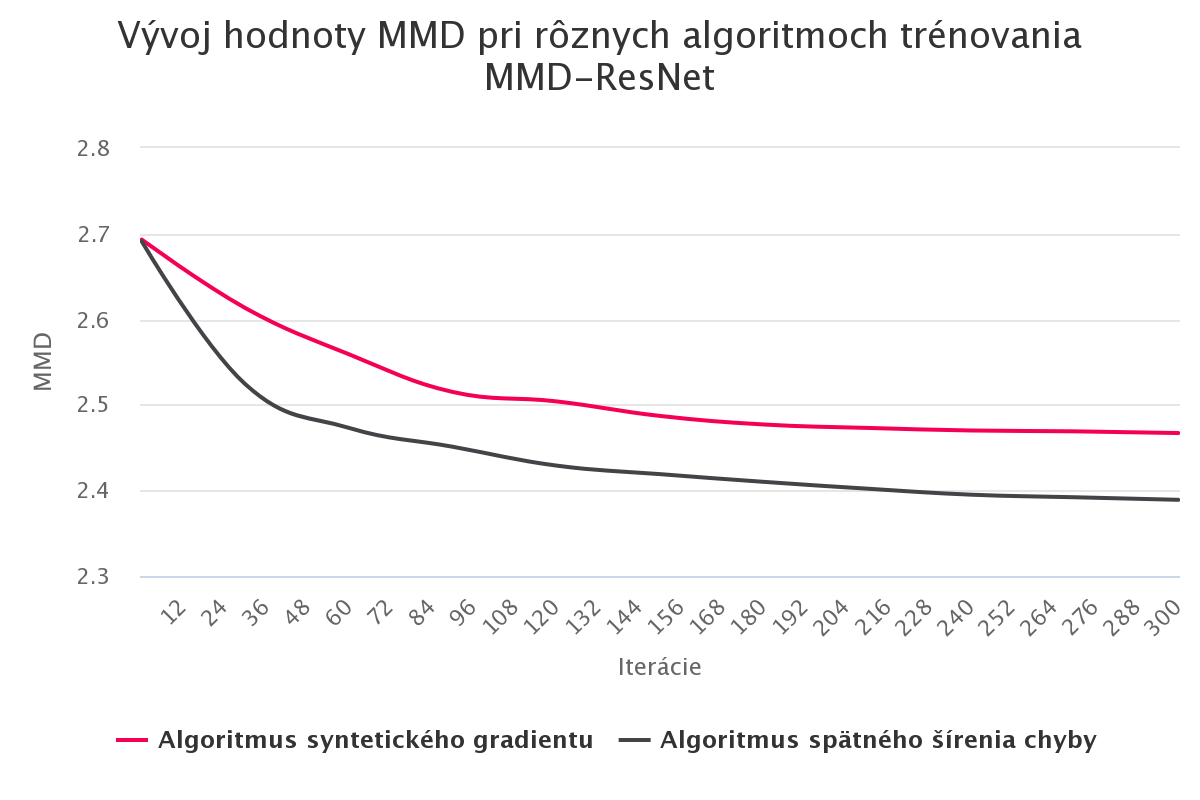
\includegraphics[width=0.7\textwidth]{images/experimenty/experiment4.png}}
%popis obrazku
\caption[Vývoj hodnoty MMD pri rôznych metódach trénovania MMD-ResNet]{Graf na obrázku opisuje vývoj hodnoty MMD medzi zdrojovou vzorkou a referenčnou vzorkou v závislosti na metóde trénovania MMD-ResNet. Červená čiara opisuje vývoj hodnoty MMD v priebehu trénovania MMD-ResNet využívajúcej metódu syntetického gradientu a čierna čiara opisuje vývoj hodnoty MMD v priebehu trénovania MMD-ResNet využívajúcej metódu spätného šírenia chyby.}
%id obrazku, pomocou ktoreho sa budeme na obrazok odvolavat
\label{vysledok4}
\end{figure}

Z Obr. \ref{vysledok4} je možné vidieť, že pri trénovaní MMD-ResNet metódou syntetického gradientu nie je dosiahnutá rovnaká hodnota MMD ako pri trénovaní MMD-ResNet využívajúcej metódu spätného šírenia chyby. Tiež je možné vidieť, že v prípade trénovania MMD-ResNet metódou syntetického gradientu je nižšia miera konvergencie hodnoty MMD ako v prípade konkurenčnej metódy. MMD-ResNet využívajúca metódu syntetického gradientu vyžaduje viacej iterácií trénovania na dosiahnutie rovnakej hodnoty MMD ako MMD-ResNet využívajúca metódu spätného šírenia chyby. Problém nedosiahnutia rovnakej hodnoty MMD medzi pozorovanými modelmi je zapríčinený dynamický sa meniacou hodnotou kroku učenia. V neskorších fázach trénovania MMD-ResNet je hodnota kroku učenia tak nízka, že jednotlivé váhy skrytých vrstiev sú upravované minimálne, čo má za následok zanedbateľný vplyv na zmenu hodnoty MMD.

Toto tvrdenie sme potvrdili experimentom, pri ktorom sme pozorovali vývoj hodnoty MMD pri trénovaní rovnakých dvoch modelov MMD-ResNet ako v predchádzajúcom experimente. Rozdiel bol v hodnote rozvrhu $T$, dynamicky sa meniaceho kroku učenia. MMD-ResNet využívajúca metódu spätného šírenia chyby využíva pôvodnú hodnotu rozvrhu dynamicky sa meniaceho kroku učenia, $T=50$. V tomto prípade hodnota rozvrhu dynamicky sa meniaceho kroku učenia znamená, že každých $50$ iterácii trénovania MMD-ResNet sa hodnota kroku učenia zmení $\gamma$-násobne. Hodnotu rozvrhu $T$ v prípade MMD-ResNet využívajúcej metódu syntetického gradientu sme zvýšili o 50\%, teda $T=75$. Výsledky experimentu je možné vidieť na Obr. \ref{vysledok5}.

\begin{figure}
%vlozenie samotneho obrazku vycentrovaneho a vhodnej velkosti
%obrazok je v subore images/cervik.png
\centerline{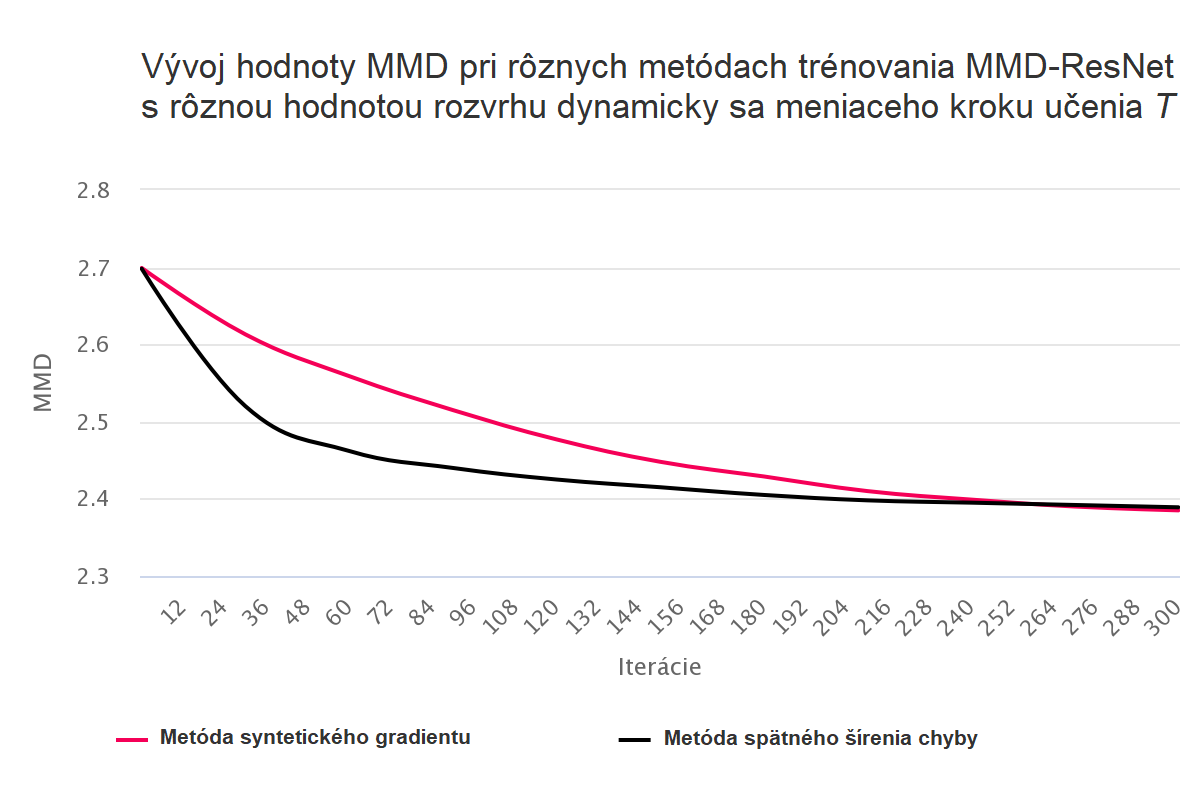
\includegraphics[width=0.7\textwidth]{images/experimenty/experiment5.png}}
%popis obrazku
\caption[Vývoj hodnoty MMD pri rôznych metódach trénovania MMD-ResNet s rôznou hodnotou rozvrhu dynamicky sa meniaceho kroku učenia $T$]{Graf na obrázku opisuje vývoj hodnoty MMD medzi zdrojovou vzorkou a referenčnou vzorkou v závislosti na metóde trénovania MMD-ResNet. Jednotlivé metódy trénovania MMD-ResNet využívajú rôznu hodnotu rozvrhu dynamicky sa meniaceho kroku učenia $T$. Pre MMD-ResNet využívajúca metódu spätného šírenia chyby sa $T=50$ a pre MMD-ResNet využívajúca metódu syntetického gradientu sa $T=75$.}
%id obrazku, pomocou ktoreho sa budeme na obrazok odvolavat
\label{vysledok5}
\end{figure}

Z Obr. \ref{vysledok5} je možné vidieť, že MMD-ResNet využívajúca metódu syntetického gradientu je vo viacerých iteráciách trénovania schopná dosiahnuť rovnakú hodnotu MMD ako MMD-ResNet využívajúca metódu spätného šírenia chyby. Ak uvažujeme optimálnu hodnotu MMD rovnú $2,415$, tak MMD-ResNet využívajúca metódu spätného šírenia chyby je schopná dosiahnuť túto hodnotu po 150 iteráciách, zatiaľ čo MMD-ResNet využívajúca metódu syntetického gradientu vyžaduje až 200 iterácií na dosiahnutie danej hodnoty. Optimálne hodnota v tomto kontexte predstavuje pomyselný bod, v ktorom sa jednotlivé modely MMD-ResNet \textit{„prestávajú učiť“}, resp. zmena hodnoty chybovej funkcie (hodnota MMD) naberá stagnujúci trend. Optimálna hodnota bola v našom prípade odhadnutá metódou lakťa.

\section{Vývoj hodnoty MMD v závislosti od času trénovania}
\label{vyvoj_MMD_v_case}

Experiment uvedený v kapitole \ref{prve_vysledky} preukázal zníženie času potrebného na trénovanie MMD-ResNet v prípade využitia metódy syntetického gradientu. Nasledujúce pozorovanie porovnáva vývoj hodnoty MMD v čase trénovania MMD-ResNet využívajúcej metódu syntetického gradientu a MMD-ResNet využívajúcej metódu spätného šírenia chyby. V danom pozorovaní mali obidva modely rovnakú konfiguráciu (opísanú v úvode Kap. \ref{vysledky}), s výnimkou trénovacej metódy a hodnoty rozvrhu dynamicky sa meniaceho kroku učenia (prevzaté z experimentu opísaného v Kap. \ref{vyvoj_MMD_v_iteraciach}). Výsledok pozorovania opisuje vývoj hodnoty MMD v čase trénovania modelov MMD-ResNet pri 300 iteráciách trénovania (viď Obr. \ref{vysledok6}).

\begin{figure}
%vlozenie samotneho obrazku vycentrovaneho a vhodnej velkosti
%obrazok je v subore images/cervik.png
\centerline{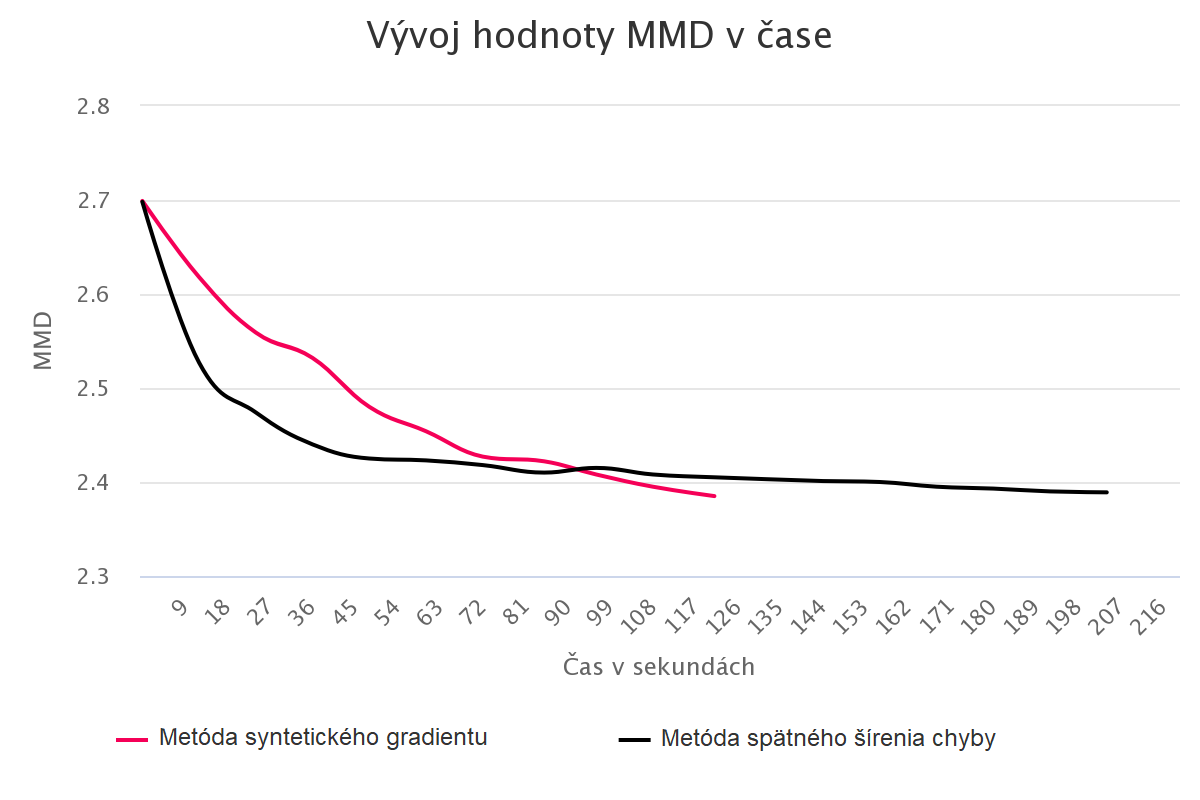
\includegraphics[width=0.7\textwidth]{images/experimenty/experiment6.png}}
%popis obrazku
\caption[Vývoj hodnoty MMD v čase trénovania]{Graf na obrázku opisuje vývoj hodnoty MMD v čase trénovania MMD-ResNet v závislosti na metóde trénovania MMD-ResNet. Jednotlivé metódy trénovania MMD-ResNet využívajú rôznu hodnotu rozvrhu dynamicky sa meniaceho kroku učenia $T$. Pre MMD-ResNet využívajúcej metódu spätného šírenia chyby sa $T=50$ a pre MMD-ResNet využívajúcej metódu syntetického gradientu sa $T=75$. Trénovanie MMD-ResNet s využitím metódy syntetického gradientu pri 300 iteráciách trvalo 121 sekúnd, pričom trénovanie MMD-ResNet s využitím metódy spätného šírenia chyby trvalo 205 sekúnd.}
%id obrazku, pomocou ktoreho sa budeme na obrazok odvolavat
\label{vysledok6}
\end{figure}

Na základe výsledkov pozorovania (Obr \ref{vysledok6}) je možné vidieť, že trénovanie MMD-ResNet s využitím metódy syntetického gradientu trvalo kratšie (121 sekúnd) ako trénovanie MMD-ResNet s využitím metódy spätného šírenia chyby (205 sekúnd). Dôležité je všimnúť si, v akom čase jednotlivé modely dosiahli optimálnu hodnotu MMD, $2,415$. Trénovanie MMD-ResNet metódou spätného šírenia chyby trvalo síce 205 sekúnd ale optimálna hodnota MMD bola dosiahnutá už po 95 sekundách. MMD-ResNet využívajúca metódu syntetického gradientu dosiahla optimálnu hodnotu MMD po 90 sekundách (viď Tab. \ref{vysledok6b}).

\begin{table}[h!]
% v tabulke sa popis zvykne davat nad tabulku
\caption[Dosiahnutie optimálnej hodnoty MMD rôznymi metódami trénovania MMD-ResNet]{Tabuľka opisuje počet iterácií a čas potrebný na dosiahnutie optimálnej hodnoty $MMD=2,415$, rôznymi metódami trénovania MMD-ResNet.}
%id tabulky
\label{vysledok6b}
% tu zacina samotna tabulka
\begin{center}
\begin{tabular}{|c|c|c|}
\hline
 Optimálna hodnota & \textbf{Metóda} & \textbf{Metóda} \\
 $MMD=2,415$ & \textbf{syntetického gradientu} & \textbf{spätného šírenia chyby} \\
\hline
\textbf{Počet iterácií} & 201 & 150 \\
\hline
\textbf{Čas} & 90s & 95s \\
\hline
%(many lines omitted)
\end{tabular}%
\end{center}
\end{table}

\section{Vývoj \textit{F1 skóre} v závislosti od iterácii trénovania}
\label{vyvoj_F1_skore_kapitola}

V kapitole \ref{navrh} sme uviedli štatistický test, ktorým je možné preukázať presnosť kalibrácie MMD-ResNet. Štatistický test vyhodnotenia presnosti kalibrácie MMD-ResNet využíva metriku \textit{F1 skóre}. Po ukončení trénovania MMD-ResNet je zdrojová vzorka použitá na kalibráciu natrénovaným modelom MMD-ResNet. Kalibrovaná zdrojová vzorka je následne gatovaná natrénovaným bunkovým klasifikátorom. Výsledok automatického gatovania kalibrovanej vzorky je porovnávaný s výsledkom manuálneho gatovania danej vzorky. Pri porovnávaní výsledkov automatického a manuálneho gatovania je vypočítaná hodnota \textit{F1 skóre} definovaná ako opisuje Kap. \ref{navrh}.

Naša implementácia MMD-ResNet zahŕňa vyhodnocovanie \textit{F1 skóre} v priebehu trénovania MMD-ResNet. Vyhodnocovanie modelu je realizované na validačných dátach, ktoré sú oddelené od trénovacích dát pred zahájením trénovania. Pri realizovaní pozorovania vývoja \textit{F1 skóre} sme implementovali jednoduchý mechanizmus ladenia hyperparametrov (konfigurácie) MMD-ResNet.

Prvotné výsledky pozorovania preukazovali 70\% úpadok \textit{F1 skóre} automatického gatovania vzorky kalibrovanej pomocou MMD-ResNet využívajúcej metódu syntetického gradientu v porovnaní s automatickým gatovaním vzorky kalibrovanej pomocou MMD-ResNet využívajúcej metódu spätného šírenia chyby. Pri hlbšej analýze sme identifikovali problém pretrénovania klasifikátora vykonávajúceho automatické gatovanie kalibrovaných vzoriek. Pretrénovanie klasifikátora spočívalo v klasifikovaní všetkých buniek do majoritnej triedy. Daný problém sme vyriešili vyvážením zastúpenia buniek jednotlivých tried v referenčnej vzorke, ktorá je používaná na trénovanie klasifikátora. Implementáciou funkcie vyváženia referenčnej vzorky bolo dosiahnuté zvýšenie \textit{F1 skóre} až o 40\%.

Aj napriek zvýšeniu \textit{F1 skóre} pomocou vyváženia referenčnej vzorky boli výsledky nedostatočné. Implementáciou jednoduchého ladenia hyperparametrov (konfigurácie) MMD-ResNet sa podarilo dosiahnuť výsledky konkurencieschopné pôvodnej implementácii MMD-ResNet. Najlepšie \textit{F1 skóre} bolo dosiahnuté pri gatovaní vzorky kalibrovanej pomocou MMD-ResNet s krokom učenia $10^{-2}$ a deaktivovaným rozvrhom dynamicky sa meniaceho kroku učenia (viď Tabuľku \ref{vysledok7b}). Výsledky pozorovania vývoja \textit{F1 skóre} v priebehu trénovania MMD-ResNet metódou syntetického gradientu je možné vidieť na obrázku \ref{vysledok7}.

\begin{figure}
%vlozenie samotneho obrazku vycentrovaneho a vhodnej velkosti
%obrazok je v subore images/cervik.png
\centerline{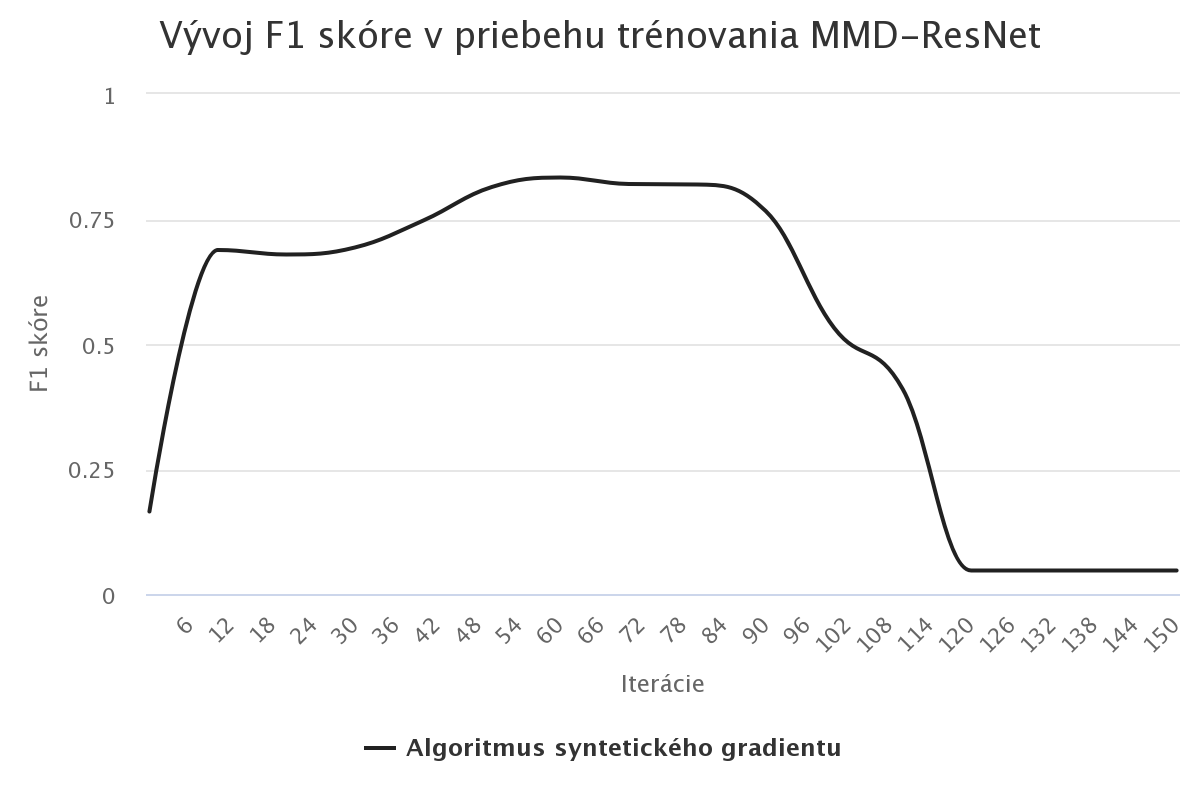
\includegraphics[width=0.7\textwidth]{images/experimenty/experiment7.png}}
%popis obrazku
\caption[Vývoj \textit{F1 skóre} v priebehu trénovania MMD-ResNet]{Graf na obrázku opisuje vývoj \textit{F1 skóre} v závislosti od iterácii trénovania MMD-ResNet využívajúcej metódu syntetického gradientu. MMD-ResNet je trénovaná krokom učenia rovným $10^{-2}$ a deaktivovaným rozvrhom dynamicky sa meniaceho kroku učenia. Maximálna hodnota \textit{F1 skóre} (0.833) je dosiahnutá už po 60 iteráciách trénovania.}
%id obrazku, pomocou ktoreho sa budeme na obrazok odvolavat
\label{vysledok7}
\end{figure}

\begin{table}[h!]
% v tabulke sa popis zvykne davat nad tabulku
\caption[Porovnanie \textit{F1 skóre} v závislosti od rôznych metód trénovania MMD-ResNet]{Tabuľka opisuje počet iterácií potrebných na dosiahnutie maximálnej hodnoty \textit{F1 skóre} v závislosti od metódy trénovania MMD-ResNet.}
%id tabulky
\label{vysledok7b}
% tu zacina samotna tabulka
\begin{center}
\begin{tabular}{|c|c|c|}
\hline
  & \textbf{Metóda} & \textbf{Metóda} \\
  & \textbf{syntetického gradientu} & \textbf{spätného šírenia chyby} \\
\hline
\textbf{Počet iterácií} & 60 & 500 \\
\hline
\textbf{\textit{F1 skóre}} & 0.833 & 0.976 \\
\hline
%(many lines omitted)
\end{tabular}%
\end{center}
\end{table}